\documentclass[12pt, a4paper]{report}
\usepackage{lmodern}
\usepackage[T1]{fontenc}
\usepackage[czech]{babel}
\usepackage[utf8]{inputenc}
\usepackage{graphicx}
\usepackage{hyperref}
\usepackage{color}
\usepackage{xcolor}
\usepackage{listings}
\lstloadlanguages{Ruby}
\lstset{language=Ruby,
	basicstyle=\ttfamily\color{black},
	commentstyle = \ttfamily\color{red},
	keywordstyle=\ttfamily\color{blue},
	stringstyle=\color{orange},
	numberstyle=\footnotesize,
	basicstyle=\ttfamily\footnotesize,
	breaklines=true,
	showspaces=false             
	language=ruby,
        basicstyle=\scriptsize
}
\lstdefinelanguage{JavaScript}{
  keywords={typeof, new, true, false, catch, function, return, null, catch, switch, var, if, in, while, do, else, case, break},
  keywordstyle=\color{blue}\bfseries,
  ndkeywords={class, export, boolean, throw, implements, import, this},
  ndkeywordstyle=\color{darkgray}\bfseries,
  identifierstyle=\color{black},
  sensitive=false,
  comment=[l]{//},
  morecomment=[s]{/*}{*/},
  commentstyle=\color{purple}\ttfamily,
  stringstyle=\color{red}\ttfamily,
  morestring=[b]',
  morestring=[b]"
}
\usepackage{caption}
\DeclareCaptionFont{white}{\color{white}}
\DeclareCaptionFormat{listing}{\colorbox{gray}{\parbox{\textwidth}{#1#2#3}}}
\captionsetup[lstlisting]{format=listing,labelfont=white,textfont=white}

\hypersetup{
	colorlinks=true,
	linkcolor=black,
	urlcolor=blue
}
\begin{document}
\author{Jan Strnádek}
\date{10.10.2012}
\title{KIV/PRJ5\\SID\\\small{SQL Injection Attack Detector\\Tento program je určen pouze k školním a testovacím účelům! Je zakázáno ho využívat k nelegální činnosti a autor ani ZČU nenese jakoukoliv zodpovědnost škodám způsobeným využitím softwaru a ani jeho součástí pro nelegální účely}}
\begin{titlepage}
\begin{center}
\textsc{\Large Západočeská Univerzita v Plzni}
\\[0.3cm]
\textsc{\Large Fakulta Aplikovaných Věd}
\\[0.3cm]
\textsc{\Large Katedra Informatiky a výpočetní techniky}
\\[6cm]
\textbf{\LARGE Bakalářská Práce}
\\[3cm]
\textbf{\LARGE SID\\[0.3cm] SQL Injection Attack Detector}
\\[6cm]
\begin{minipage}{0.4\textwidth}
\begin{flushleft}
\large
Plzeň, 2013
\end{flushleft}
\end{minipage}
\begin{minipage}{0.4\textwidth}
\begin{flushright} 
Jan Strnádek
\end{flushright}
\end{minipage}
\vfill
\end{center}
\end{titlepage}
\tableofcontents
\newpage
% Prohlaseni
\thispagestyle{empty}
\subsection*{Poděkování}
Rád bych touto cestou poděkoval Ing. Pavlu Královi, Ph.D. za odborné vedení a podnětné rady k bakalářské práci, dále pak panu Josefu Šimánkovi za odborné konzultace týkající se vývoje v Ruby a doporučení použitých knihoven.
\\[9cm]
\subsection*{Čestné prohlášení}
Prohlašuji, že svou bakalářskou práci na téma \uv{SID - SQL Injeciton Detector} jsem vypracoval samostatně pod vedením vedoucího bakalářské práce a s použitím odborných zdrojů a literatury, které jsou citovány a uvedeny v seznamu literatury, popřípadě u některých zdrojů přímo v textu. Jako autor práce dále prohlašuji, že jsem v souvislosti s jejím vytvořením neporušil autorská práva třetích osob.
\\[1.5cm]
\begin{minipage}{0.4\textwidth}
\begin{flushleft}
V Plzni dne 7.5.2013
\end{flushleft}
\end{minipage}
\begin{minipage}{0.6\textwidth}
\begin{flushright} 
$\_\_\_\_\_\_\_\_\_\_\_\_\_\_\_\_\_$
\end{flushright}
\end{minipage}
\newpage
\thispagestyle{empty}
\section*{Abstrakt}
\subsection*{English}
The main issue of this bachelor thesis is the analysis of the most recent attacks on web sites and web applications. In the theoretical part of this thesis chosen cases of attacks have been thoroughly investigated and compared and the methods of prevention have been proposed. These methods cover wide range of possible attacts both with and without frameworks. \\
The practical part has been focused on development of the penetration test for detection of one of the most dangerous security risk - SQL Injection. The suggested penetration test uses parameters that are automatically changeable to be fitted for the certain web site or application. The changes in the web site or web application are recorded and compared.\\
The proposed penetration test have been tested and compared with existing tools. Unfortunately, there has been found no similar tool available for free with direct detection function for SQL Injection, therefore the most similar freeware tools trying to test this security threat have been used for the comparison.

\subsection*{Česky}
Tato bakalářská práce se zabývá analýzou nejběžnějších útoků na webové stránky a aplikace, jejich porovnání, ukázkou a rozebrání možností zabezpečení při použití stadartního jazyka nebo při využití různých frameworkových nástrojů.\\
Druhá praktická část se zabývá vytvořením nástroje (penetračního testu) pro odhalení jednoho z největších bezpečnostních rizik - SQL Injection. Penetrační test využívá automatické úpravy parametrů v požadavcích na webovou aplikaci a porovnávání změny obsahu stránky.\\
Ve třetí části je výsledný test srovnáván s existujícími nástroji a porovnávány výsledky, bohužel k absenci podobného nástroje, který by byl zdarma je porovnáván s \uv{podobnými} nástroji, které se o detekci snaží.



\chapter{Úvod}
V dnešní době je internet synonymem pro používání počítače, tabletu, smartphone a jiných zařízení. S tím rozhodně souvisí otázka bezpečnosti uživatelských dat. Většina uživatelů bohužel využívá všude stejné heslo, proto obezřetnému hackerovi stačí získat login a heslo z jedné databáze a zkusit to i jinde. K této situace došlo nedávno při napadení pornostránek (\textit{http://pron.com}) skupinou \uv{LulzSec}\footnote{Lulz Security - tato skupina stála i za útokem na Sony Pictures v roce 2011, kde právě díky SQL Injection odcizila velké množství dat.}, která následně získaná data zveřejnila. Hesla nebyla v databázích nijak \uv{hashována}\footnote{Hash - algoritmus pro převedení vstupních dat do unikátního otisku, tato funkce \uv{by měla být jednosměrná!}}, byla uložena v podobě otevřeného textu, a proto nebyl problém vyzkoušet se přihlásit do emailových schránek, popřípadě dalších jiných webových služeb, které tito uživatelé využívali. Nikdy přesně nevíme, komu vlastně data svěřujeme a jaké bezpečnostní opatření je dotyčnou firmou či osobou zajištěno! Data jsou uchováváná v mnoha databázových systémech a jednou z hlavních otázek je také bezpečnost těchto dat. Možností útoků na webové applikace, webové stránky nebo přímo servery je mnoho. Významnější budou popsány v následující kaptiole.\\
Cílem této práce je seznámení čtenáře s bezpečnostními riziky webových aplikací a jak jim předejít, dále podrobnější seznámení s problémem SQL injection a v praktické části vytvořením nástroje pro penetrační testy na detekci těchto bezpečnostních rizik.\\
Celá tato práce je především zaměřena na detekci problému SQL injection. Aktuálně je podle serveru \uv{http://techworld.com} za zhruba 97\% úniků dat zneužití právě této chyby. 

\chapter{Útoky na webové aplikace}
\section{Přehled}
Přehled typů útoků, které budou dále detailně rozebrány.
\begin{itemize}
\item XSS - Cross-Site scripting
\begin{itemize}
\item Využití nechráněných vstupů pro vložení vlastního JavaScriptového kódu.
\end{itemize}
\item DT - Directory traversal
\begin{itemize}
\item Získávání zdrojových souborů přes špatně nastavené direktivy.
\end{itemize}
\item CSRF - Cross-Site Request Forgery 
\begin{itemize}
\item Volání nelegitimních akcí z legitmního zdroje.
\end{itemize}
\item PHP remote upload and execution scripts
\begin{itemize}
\item Zneužití nahrávaných souborů přes webové formuláře.
\end{itemize}
\item SQL Injection - normal / blind
\begin{itemize}
\item Úpravy databázových dotazů přes neochráněné vstupy.
\end{itemize}
\item a další, protože webový server je jen počítačs operačním systémem, který obsahuje bezpečnostní chyby
\end{itemize}

\section{Nejčastější typy útoků}
Se zajímavými daty přichází server \textit{http://cnet.com}, který uvádí, že každé 2 minuty je napadnuta nějaká webová stránka. Zastoupení typů provedených útoků je vidět na následujícím grafu \ref{chart.attack_list}.

\begin{figure}[h!]
\centerline{\includegraphics[width=250px]{./examples/chart.png}}
\caption{Graf nejčastějších typů útoků [Zdroj: \textit{http://cnet.com}]}
\label{chart.attack_list}
\end{figure}


\section{XSS - Cross-Site scripting}
XSS využívá podobně jako SQLi neochráněných vstupních proměnných na webových stránkách. Díky nim může do aplikací podstrčit svůj vlastní (například JavaScriptový) kód, což může následně využít k získání dat (zejména cookies od uživatelů), znedostupnění webových stránek atd. Existují dva základní typy XSS útoku:

\subsection{Nepersistentní}
Tento typ využívá nezabezpečených vstupních proměnných z URL adresy / POST dat\footnote{GET a POST jsou základní způsoby jak přenést parametry na další stranu, rozdíl je v tom, že GET jsou vidět v URL a POST ne. Ale oba dva lze bez problémů podvrhovat!}, které jsou vypisovány na stránku. Útočníkovi stačí URL upravit a nějakým způsobem (například sociálním inženýrstvím, podvrženým emailem z banky apod.) donutit uživatele na tento odkaz kliknout. 

\subsection{Persistentní}
Tento typ je mnohem nebezpečnější, protože na napadné stránky se nevstupuje přes upravenou URL adresu, ale kód se vykonává automaticky. Tato chyba se často objevuje v různých diskusních fórech či návštěvních knihách, kde se nevalidují vstupy. Do těchto nezabezpečených vstupů stačí účtočníkovi pouze vložit Java Scriptový kód, který se následně provede každému, kdo tuto stránku otevře. 

\subsection{Ukázka}
Na obrázku \ref{obr.airbank} můžeme vidět úspěšný nepersistentní XSS útok na serveru air/bank. V nechráněném vstupu byl zadán kód výstražné hlášky javascriptu:
\begin{lstlisting}[label=some-code, language=HTML, caption=Výstražná hláška v jazyce JavaScript]
<script type="text/javascritpt">alert("XSS by PiratezSec");</script>
\end{lstlisting}

\begin{figure}[h!]
\includegraphics[width=390px]{./examples/xss-airbank.png}
\caption{Non-persistent XSS}
\label{obr.airbank}
\end{figure}

Tato chyba byla objevena skupinou Czechurity (\textit{https://twitter.com/Czechurity}), která má na svědomí i kompromitaci webových stránek Unicredit bank v březnu 2013, které bylo médii chybně interpretováno jako DDoS\footnote{Distributed Denial of Service - útok, který zahlcuje službu, až dojde k jejímu pádu nebo nedostupnosti pro ostatní uživatele.}.

\subsection{Různé varianty zapsání XSS}
Výstupy na webových stránkách mohou být různým způsobem filtrovány, popřípadě může být přímo filtrován script tag. Toto lze bohužel jednoduše obejít. Zde několik příkladů (ale ne všechny prohlížeče toto interpretují):

\begin{lstlisting}[label=some-code, language=HTML, caption=Schování JavaScriptu do neexistujícího obrázku]
<img src="javascript:alert('XSS');">
\end{lstlisting}

\begin{lstlisting}[label=some-code, language=HTML, caption=Zakázané uvozovky? Nahrazení entitami \ldots]
<img src=javascript:alert(\&quot;XSS\&quot;)>
\end{lstlisting}

\begin{lstlisting}[label=some-code, language=HTML, caption=Další možností je převedení na unikód]
<img src=&#106;&#97;&#118;&#97;&#115;&#99;&#114;&#105;
&#112;&#116;&#58;&#97;&#108;&#101;&#114;&#116;&#40;
&#39;&#88;&#83;&#83;&#39;&#41;>
\end{lstlisting}

\subsection{Obrana}
Obrana před XSS není snadná. Velké webové portály mají desítky různých vstupů, které je třeba hlídat. Pokud se rozhodneme využít nějaký framework, pak je ideální obranou výběr takového, který právě těmto incidentům dovede předcházet (Nette Framework\footnote{http://nette.org}, Ruby on Rails\footnote{http://rubyonrails.org} apod.). Dále je kvůli zamezení persitentním útokům třeba striktně hlídat, co ukládáme do databází či do jiných úložišť.

\subsection{Důsledky}
Asi nejzásadnějším důsledkem úspěšného XSS útoku bude tzv. \textit{sessions hijacking}. Je to odcizení sessions$\_$id (sessions$\_$key), což je unikátní ID uživatele pro přihlašování ke vzdáleným serverům. Toto ID je možné zjistit několika způsoby, ale nejúčinějším způsobem, jak jej zjistit, je právě pomocí XSS. Pokud útočník toto ID získá, může se autorizovat k zabezpečenému serveru.

\section{Directory traversal}
Webový server slouží hlavně pro poskytování souborů, které mohou být statické (obrázky, css styly, HTML soubory) nebo dynamické (Ruby, PHP, ASP atd.). Pokud vytvoříme požadavek na web server, pak nám server při statickém obsahu soubor okamžitě interpretuje, ale při dynamickém ho nejdříve zpracuje a pak interpretuje. Při útoku typu \uv{directory traversal} využívá útočník špatného či dokonce žádného omezení přístupu k souborům právě pomocí dynamického obsahu webového serveru.

\subsection{Příklad directory traversal útoku}
Mějme:
\begin{lstlisting}[label=some-code,caption=URL adresa s podezdřením na include souboru]
http://portal.czu.cz/index.php?item=novinky.html
\end{lstlisting}
Při bližším zkoumání vidíme, že se zde pravděpodobně vkládá soubor \uv{novin ky.html} do stránky, a to odněkud ze souborového systému. Otázkou však zůstává, co se bude dít, budeme-li tento parametr měnit ručně, a kam až se dostaneme.

\begin{lstlisting}[label=man_url_get_htaccess,caption=Manipulace s URL - získání .htaccess]
http://portal.czu.cz/index.php?item=../.htaccess
\end{lstlisting}

\begin{lstlisting}[label=man_url_get_neon,caption=Manipulace s URL - získání config.neon]
http://portal.czu.cz/index.php?item=../config/config.neon
\end{lstlisting}

V prvním příkladě jsme se snažili získat soubor \uv{.htaccess}, který může obsahovat autentizační metody, nastavení práv apod. Ve druhém příkladě jsme se poukoušeli získat soubor \uv{config.neon}. Tento soubor slouží pro uchování citlivých informací na webech, které využívají Nette Framework. Příkladem takových informací může být přihlášení k databázi.

\subsection{IIS Web Server}
Starší verze IIS\footnote{Internet Information Service - Microsoftem distribuovaná obdoba webového serveru Apache2} umožňovaly dokonce i vykonávat příkazy na serveru.

\begin{lstlisting}[label=iis_derave,caption=Ukázka URL pro \uv{děravé} IIS]
http://iis.czu.cz/scr/..%5c../winnt/system32/ cmd.exe?/c+dir+c:\
\end{lstlisting}

Tento příkaz spustil \uv{cmd.exe} (příkazová řádka systému Windows) a v něm příkaz \uv{dir c:$\backslash$}. Nic nám tedy nebrání přidávat uživatele do systému, nebo formátovat pevné disky, jak lze vidět zde:

\begin{lstlisting}[label=iis_derave_format,caption=Formátování disku C: přes chybu v IIS]
http://iis.czu.cz/scr/..%5c../winnt/system32/ cmd.exe?/c+format+c:\
\end{lstlisting}

\subsection{Obrana}
\begin{itemize}
\item Mít správně nastavená oprávnění a cesty jednotlivých webových serverů (virtuálních hostů).
\item Kontrolovat, co vlastně do stránky vkládáme.
\item Úplně se vyhnout vkládání dat do stránky (například v PHP můžeme použít \textit{spl$\_$autoload$\_$register}, který nám automaticky podle zadané funkce načítá třídy ze souborového systému).
\end{itemize}

\subsection{Praktická ukázka}
Na obrázku \ref{obr.directory} vidíme úspěšný directory traversal útok na vkládání v parametru \uv{name}. Ze získaného souboru \uv{config.neon} se následně dozvíme, že přihlašovací jméno k databázi je \uv{franta} a heslo je také \uv{franta}.
\begin{figure}[h!]
\centerline{\includegraphics[width=380px]{./examples/dir_example.png}}
\caption{Directory traversal - zobrazení souboru config.neon}
\label{obr.directory}
\end{figure}

\section{CSRF - Cross-Site Request Forgery}
U tohoto typu útoku většinou potřebujeme \uv{osobu uvnitř}, která má dostatečná oprávnění a my jsme schopni jí přesvědčit (často pomocí sociálního inženýrství), aby spustila nebo otevřela námi upravenou URL. Tento útok využívá situace, že sice přijde požadavek na vykonání určité akce od legitmního uživatele, ale na neligitimní zdroj. (Tento postup často vyžaduje zanlost URL pro různé akce na webové stránce.)
\subsection{Příklad CSRF}
Jednoduchým příkladem může být jakýkoliv redakční systém. Nejjednoduší je, pokud server, na který útočíme, používá nějaký známý CMS\footnote{Content Managment System - systém zajišťující správu webového obsahu} - například Joomla\footnote{http://www.joomla.org/ - PHP CMS}, Drupal\footnote{http://www.drupal.org/ - Open CMS system} a další. Zde URL adresy pro vykonávání určitých akcí známe, protože si je můžeme vyzkoušet sami. Mějme tedy redakční systém, který má script \textit{admin.php} a například tyto parametry:
\begin{itemize}
\item \textbf{action} - Která akce bude provedena
\item \textbf{user} - Uživatel
\item \textbf{hodnota} - Nějaká další hodnota
\end{itemize}

Můžeme tedy spustit například toto:
\begin{lstlisting}[label=csfr_example1,caption=URL změny uživatelské role]
http://portal.czu.cz/admin.php?action=changeRole&user=2&role=admin
\end{lstlisting}

Jestliže tento příkaz (\textit{změna role uživatele \uv{2}, což jsme například právě my, na roli \uv{hlavního administrátora}}) zavoláme jako neautorizovaná osoba, příkaz se neprovede a bude nám vypsáno, že nemáme dostatečná oprávnění. Jestliže ovšem zašleme podvodný email správci portálu, který na tento link klikne a bude zároveň přihlášen na zmíněné stránce {http://portal.czu.cz}, tento příkaz proběhne bez problémů, uživatel Honza bude mít práva \uv{hlavního administrátora}, což už je značný bezpečnostní problém.

\subsection{Obrana proti CSRF}
Nejúčinější obranou proti CSRF je generování a kontrolování tokenů. Do každého formuláře, popřípadě i odkazu, přidáme tzv. \uv{token} (tj. náhodně vygenerovaný řetězec, příklad URL s tokenem viz \ref{token_url}), který se uloží a následně přidá do každého formuláře / odkazu na aktuální stránce. Při přechodu na další stránku se přijatý token ověří proti uloženému. Pokud je vše v pořádku, akce se provede. Pokud token nesouhlasí, je uživatel přesměrován na \uv{bezpečnou} stránku, která jej informuje o neplatné akci. Tato metoda obrany je založena na tom, že útočník není schopen token předvídat. Samozřejmě, pokud by byla chyba při generování tokenu, popřípadě by se \\z nějakého důvodu neměnil, je zde možnost, že jej útočník zjistí.

\begin{lstlisting}[label=token_url,language=HTML, caption=CSRF obrana - token]
http://czu.cz/admin.php?action=changeRole&user=2&role=1&token=ad70CZf82
\end{lstlisting}

\section{Remote execution script}
Tento typ útoku využívá situaci, kdy můžeme pomocí formuláře pro nahrání souborů nahrát PHP skript, který je dostupný pomocí URL a je web serverem vykonáván. Správně vytvořený PHP skript pak může naše akce směrovat pomocí příkazů (system() a eval()) na konzoli stroje a následně nám umožňuje další činnost. Jednou z možností je využítí scriptu pro vytvoření reverzního shellu\footnote{Reverse Shell - otevření spojení z cílového stroje na náš počítač \uv{jakoby} SSH obráceně}. Tento script umí vytvořit například oblíbený Metasploit framework\footnote{Metasploit framework je velice oblíbený penetrační tester, který lze získat zdarma na: http://www.metasploit.com/}, který pak skýtá opravdu široké využití.

\subsection{Obrana}
Zde je obrana jednoduchá, a to dávát si pozor na to, co je nahráváno. Soubory můžeme tedy jednoduše přejmenovávat (změnit přípomnu z interpretovaných - \textit{.php}, \textit{.php3}  například na \textit{.txt}, které není interpretováno) nebo zakázat jejich vykonávání. Příklade Další užitečnou funkcí pro \uv{předejití} problémům je zákaz funkcí \textit{eval()} a \textit{system()}. Tyto funkce umožnějí volání systémových funkcí (spouštění programů, kopírování souborů atd.). Značný problém je, když webový server běží pod účtem superuživatele (\textit{root}). Útočník tedy získává automaticky práva hlavního administrátora, což může mít neblahé následky. Proto se webové servery a další služby spoušťí pod speciálními uživateli s omezenými právy.

\section{Open Directory browsing}
Další ukázka špatně nastaveného serveru. Jsme totiž schopni zjistit adresářovou strukturu projektů a z ní vyčíst mnoho informací, které měly zůstat skryty. Příkladem mohly být dříve používané soubory s příponou \textit{.inc}, které bylo možné číst, protože je PHP interpret standardně nevykonával. Tyto soubory je stále možné nalézt pomocí internetových vyhledávačů (často byly vyhledávány soubory s názvem \textit{config.php.inc}, které obsahovaly většinou údaje pro připojení k databázi a jiné konfigurační údaje).

\section{SQL Injection}
Podobně jako XSS využívá SQL injection neochráněné vstupy, ovšem využívá je jako útok na databázovou vrstvu, protože pomocí neochráněných vstupů upravuje SQL dotazy volané nad databázovým serverem. (Více o SQL injection bude rozebráno v kapitole 3)

\section{Frameworky}
Dnes jsou v oblibě frameworky pro rychlejší a snažší vývoj webů. Některé z nich kladou důraz na obranu proti XSS, CSRF i SQLi, ale lze jim věřit? U většiny frameworků je zmíněno tzv. \uv{escapování}, což znamená převedení \uv{nebezpečných znaků}: \uv{<>\"} atd. na \uv{bezpečné}, které nejsou prohlížečem nebo SQL interpretem vykonávány. Jestliže vypisujeme neescapovanou proměnnou, může to znamenat bezpečnostní riziko! Dále budou uvedeny základní bezpečnostní nedostatky některých z frameworků, které byly objeveny za posledních několik měsíců.

\begin{enumerate}
\item \textit{Zend Framework - PHP} 
\begin{itemize}
\item \textit{http://framework.zend.com/}
\item \textit{SQL Injection a XSS} - neprovádí escapování a je nutné využít další funkce (stejně jako v čistém PHP)
\item \textit{CSRF} - obrana proti CSRF je plně na bedrech programátora
\end{itemize}
\item \textit{Ruby on Rails (RoR) - Ruby}
\begin{itemize}
\item \textit{http://rubyonrails.org/}
\item \textit{SQL Injection} - 2. 1. 2013 byla objevena zásadní chyba tohoto typu v modulu Active Record, který Ruby on Rails využívá jako ORM\footnote{ORM - objektové relační mapování - mapuje data z databází na objekty}. Chybou, která byla označena jako CVE-2012-5664, jsou postiženy všechny verze Ruby on Rails: \textit{https://groups.google.com/\\forum/$\#$!topic/ rubyonrails-security/DCNTNp$\_$qjFM}. Veškeré dotazy jsou striktně escapovány, ale pro určite položky to lze vypnout tzn. položky, u kterých bylo escapování vypnuto se nebude nic ověřovat a tyto položky mohou být bezpečnostním rizikem.
\item \textit{CSRF} - Tokeny jsou přidávány ke všem formulářům automaticky od Ruby on Rails verze 2.
\item \textit{XSS} 
\begin{itemize}
\item RoR ve verzi 2 nehlídala výstupy v šablonách a bylo nutné používat helper\footnote{Jednoduché makro používané v šabloně.}.
\item RoR ve verzi 3 hlídá vše, ale je možné vynutit vypsání normální (hodí se například pokud máme \uv{před tím} postaven Markdown\footnote{Nástroj pro převádění textu do HTML pomocí speciálních značek.}, který vstup a výstup hlídá sám).
\end{itemize}
\end{itemize} 
\item \textit{DJango - Python}
\begin{itemize}
\item \textit{https://www.djangoproject.com/}
\item \textit{SQL Injection}
\begin{itemize}
\item Querysets - ORM - hlídají proměnné automaticky, lze vynutit, aby se tak nedělo
\item RAW queries - neescapují vůbec
\end{itemize}
\item \textit{CSRF} - Django obsahuje \textit{middleware}\footnote{Middleware je tzv. \uv{prostředník}, v tomto případě mezi jádrem DJanga a naší aplikací.}, který nám umožní přidávat CSRF token k formulářům a následně ho ověřovat: - víc e informcí na: \textit{https://docs.djangoproject.com/en/dev/ref/contrib/csrf/}.
\item \textit{XSS} - Šablony DJanga automaticky escapují proměnné, ale ne všechny (více informací na: \textit{https://docs.djangoproject.com/en/ dev/topics/security/}).
\end{itemize}
\item \textit{Nette Framework - PHP}
\begin{itemize}
\item \textit{http://nette.org/cs/}
\item \textit{SQL Injection}  - při využití \textit{Nette$\backslash$Database}\footnote{\textit{Nette$\backslash$Database} je název vrstvy pro jednodušší práci s databází} se escapují všechny proměnné automaticky (ovšem lze zde vynutit neescapování).
\item \textit{CSRF} - Nette$\backslash$Forms\footnote{Třída reprezentující formuláře v Nette} mají volbu zapnout přidávání CSRF tokenu a následně ho sami ověřují (pomocí metody \textit{addProtection()}).
\item \textit{XSS} - Veškeré proměnné vypisované do šablon jsou automaticky escapovány. Lze opět vynutit, aby k tomu nedocházelo.
\end{itemize}
 
\item \textit{ASP - C$\#$}
\begin{itemize}
\item \textit{SQL Injection} - Pokud je použita výchozí databázová vrstva ASP, escapuje se úplně vše a není možné tuto funkčnost vypnout. Pokud je ovšem SQL dotaz napsán ručně, je to čistě na programátorovi.
\item \textit{XSS} - Striktně se escapují všechny proměnné, které se vkládají do šablon.
\item \textit{CSRF} - Tokeny ve formulářích nejsou implicitně zapnuty, ale je možné využít \textit{ViewStateUserKey}, popřípadě knihovny třetích stran.
\end{itemize}
\end{enumerate}

\chapter{SQL Injection (SQLi)}
\section{Popis}
SQL Injection podobně jako XSS využívá neochráněných vstupů, ovšem cílem je napadání databázové vrstvy (viz dříve). Pomocí neochráněných vstupů jsme schopni upravovat SQL dotazy, vkládat do nich podmínky, popřípadě vnořené dotazy.

\section{Příklad SQL Injection}
Mějme tabulku (například v databázovém systému \textit{MySQL}) se seznamem písniček. Ukázku tabulky můžeme vidět v tabulce:
\begin{table}[!h]
\centering
\begin{tabular}{|c|c|l|l|}
\hline
\bf id & \bf category$\_$id & \bf autor & \bf name \\
\hline
\hline
\bf 1. & \bf 2 & Celldweller & One good reason \\
\hline
\bf 2. & \bf 3 & Asonance & Království Keltů \\
\hline
\bf 3. & \bf 2 & Celldweller & EON \\
\hline
\bf 4. & \bf 4 & Hectix & Return \\
\hline
\bf 5. & \bf 3 & Blue Stahli & Takedown\\
\hline
\end{tabular}
\label{tab:hac}
\caption{Tabulka hudebního katalogu}
\end{table}
\newline
Ve webové aplikaci přejdeme na URL:
\begin{lstlisting}[label=web_app_url_1,language=HTML, caption=URL webové aplikace]
http://localhost/songs.php?categoryId=2
\end{lstlisting}

Script \textit{songs.php} načte parametr \textit{categoryId} a podle něj vytvoří dotaz, který vybere písničky z dané kategorie:

\begin{lstlisting}[label=web_app_url_2,language=SQL, caption=Vytvořený SQL dotaz]
SELECT * FROM songs WHERE category_id = 2
\end{lstlisting}

Dotaz bude vykonán a na webové stránce se zobrazí pouze písničky z kategorie číslo 2. Pokud bychom ale URL ručně přepsali a nahradili bychom kritickou část, například:
\begin{lstlisting}[label=web_app_url_3,language=HTML, caption=Ručně upravené URL]
http://localhost/songs.php?categoryId = 2 OR 1 = 1
\end{lstlisting}

a script by nebyl ochráněn proti těmto \uv{nevhodným} vstupům, zachoval by se stejně a vygeneroval by následující dotaz:
\begin{lstlisting}[label=web_app_url_4,language=SQL, caption=Vygenerovaný SQL dotaz z upraveného URL]
SELECT * FROM songs WHERE category_id = 2 OR 1 = 1
\end{lstlisting}

Tento dotaz je ovšem úplně jiný, vrací totiž všechny skladby.

\section{Rozdíl mezi SQL Injection a Blind SQL Injection}
Podstata útoku je v obou případech stejná, ovšem u \textit{Blind SQL Injection} nevidíme výsledek, což znamená delší hledání problému. Oproti tomu v předchozím případě jsme výsledek viděli ihned (zobrazily se všechny skladby a ne pouze daná kategorie), což znamenalo odhalení tohoto problému. 

\section{Předcházení a obrana}
\begin{itemize}
\item Kontrola příchozích dat na aplikační vrstvě - pokud vím, že mi v parametru \textit{category\_id} má přijít číslo, tak budu validovat číslo.
\item Využití funkcí pro \uv{přepsání} speciálních znaků do entit (v php např.: \textit{mysql\_real\_escape\_string} \ldots). Tyto funkce nahradí znaky, které by mohly SQL dotaz nějakým způsobem \textit{upravit} nebo \textit{poškodit} na text.
\item Využití databázové vrstvy, která má jako jeden z cílů právě předcházení těmto rizikům (příkladem může být \textit{Dibi - Database Abstraction Library pro PHP}\footnote{Je zdarma k dispozici na http://dibiphp.com}).
\item Správně nastavená oprávnění - pro připojení webových aplikací využívat speciálního uživatele s omezenými právy (pokud je z nějakého důvodu nepotřebujeme). Ideálně aplikace a k ní konkrétní uživatel s jednou databází, který nikam jinam nemůže (zabránění, aby se z DB jedné aplikace dostal i do dalších), dále zakáz nepotřebných příkazů pro tyto uživatele (například exec, drop, alter). Pak i kdyby útočník objevil SQL Injection chybu, tak nám například nemůže vymazat všechny tabulky.
\end{itemize}

\chapter{Důsledky}
Důsledky napadení nedostatečně zabezpečené aplikace mohou být fatální, ať je to získání administrátorského přístupu do webové aplikace, odcizení dat nebo až získání úplné kontroly nad cílovým serverem.

\section{Ukázky možného napadení}
\subsection{SQLi v redakčním systému}
Tato chyba byla nahlášena na \textit{http://exploit-db.org/} a její kód zveřejněn. Byly zasaženy desítky webů používajících redakční systém WordPress. Z obrázku je vidět, že parametr \textit{id} není bezpečný, tudíž je možné dotaz upravit a získat například uživatelská jména či  hesla.
\begin{figure}[h!]
\centering{\includegraphics[width=390px]{./examples/squash-sqli.png}}
\caption{SQL injection v redakčním systému}
\label{obr.squash}
\end{figure}

\subsection{Chybný přihlašovací formulář}
Ukázka chybně zabezpečného vstup přihlašovacího formuláře na nejmenovaném portálu české firmy, kde je možné se pomocí zakomentování zbytku SQL dotazu (ověření hesla) přihlásit jako administrátor.
\begin{figure}[h!]
\centering{\includegraphics[width=282px]{./examples/login_test.png}}
\caption{Zápis SQLi}
\label{obr.login1}
\end{figure}

\begin{figure}[h!]
\centering{\includegraphics[width=346px]{./examples/login_suc.png}}
\caption{Úspěšné přihlášení}
\label{obr.login2}
\end{figure}


\subsection{Sony Pictures - 2011}
Proti společnosti Sony byly v roce 2011 několikrát použity DDoS útoky a nakonec vše vyústilo v odcizení dat skupinou LulzSec\footnote{Lulz Security - skupina počítačových hackerů, jejich webové stránky byly zablokovány, ale twitter zůstal \textit{https://twitter.com/LulzSec}} pomocí SQL injection. I taková velká společnost jako sony, měla údaje v databázích v nešifrované podobě. Hackerům se podařilo odcizit 1 milion uživatelských dat (jména, hesla, adresy a datumy narození), dále hesla administrátorů a mnoho dalšího - více v \textit{http://www.thewhir.com/web-hosting-news/hackers-attack-sony-pictures-with-single-sql-injection}. Tato skupina byla nedávno zatčena díky chybě a následné spolupráci jejich hlavního člena.

\begin{center}
\textit{You call it war, we laugh at your battleships.}\\
(Heslo skupiny LulzSec)
\end{center}

\chapter{Návrh nástroje pro penetrační testování}

\section{Postup testu}
\begin{enumerate}
\item Analýza zdrojového kódu 
\begin{itemize}
\item Získání objektové reprezentace webové stránky použitelné pro další zpracování.
\end{itemize}
\item Vytvoření stromu webové stránky
\begin{itemize}
\item Extrahování formulářů a hypertextových odkazů z webové stránky (pro vytvoření stromu).
\item Normalizace URL adres kvůli detekování přechodu na jiné domény a sjednocení všech možných kombinací relativních a absolutních URL adres.
\end{itemize}
\item Otestování hypertextových odkazů
\begin{itemize}
\item Otestování možnosti SQLi v hypertextových odkazech pomocí analýzy webové stránky (změna stránky - počtu elementů v závislosti na úpravě sql dotazu).
\end{itemize}
\item Otestování formulářů
\begin{itemize}
\item Stejný postup jako u hypertextových odkazů.
\end{itemize}
\item Reprezentace výsledků
\begin{itemize}
\item Reprezentace výsledků pro další zpracování - na standardní výstup, popřípadě ve specifickém formátu do souboru.
\end{itemize}
\end{enumerate}

\section{Analýza zdrojového kódu stránky}
Při analýze stojí za úvahu, zda si napsat vlastní HTML parser nebo použít nějaký stávající, čímž by bylo rozhodnuto i o jazyce, ve kterém bude testovací script napsán. Bylo možné použít  následující HTML parsery:
\begin{itemize}
\item XML Reader - PHP
\item Simple HTML DOM - PHP
\item Nokogiri - Ruby
\item Hpricot - Ruby
\item JSoup - Java
\end{itemize}

\subsection{Testování parserů}
Pro testování jsem si napsal 2 webové stránky, první s validním a správně napsaným HTML a druhou s rozházenými tagy, nedokončenými uvozovkami, která by měla více reprezentovat reálný model webových stránek. I když existují xHTML standardy je většina projektů psaná \uv{ve spěchu} a kód bývá dost často nepořádný. Proto je nutné tento problémem zohlednit.\\
\newline
\textbf{XML Reader - PHP} - Tento parser je primárně pro parsování validních XML dokumentů, proto se ukázal pro parsování HTML stránek jako nevhodný.\\
\textit{(Ke stažení na: http://php.net/manual/en/book.xmlreader.php)}\\
\newline
\textbf{Simple HTML DOM - PHP} - Parser v PHP určený přímo pro parsování HTML DOM Modelu se jevil jako vhodný kandidát, ale při otestování na reálném webu (sestavování stromu webové stránky) se parser ukázal jako nepoužitelný. Velmi špatně reagoval na další chyby v HTML stránce a nebylo možné je rozumně zachytávat. Také jeho výběr prvků a následné parsování dat bylo nutné kombinovat s regulárními výrazy. Ze zmíněných důvodů jsem od tohoto parseru upustil.\\
\textit{(Ke stažení na: http://simplehtmldom.sourceforge.net/)}\\
\newline
\textbf{Nokogiri - Ruby} - První parser v testu, který si bez problémů poradil s parsováním špatných HTML stránek, byl schopen rozpoznat správně odkazy, chybné uzavírání parametrů. Další obrovským přínosem je, že funguje na principu CSS3 selektorů:
\begin{lstlisting}[label=some-code,language=Ruby, caption=CSS3 Selektory NokoGiri]
# Load Nokogiri::HTML Document for page
doc = Nokogiri::HTML(open('http://www.google.com/search?q=sparklemotion'))

# Search for nodes by css
doc.css("body a").each do |link|
	puts link.content
end
\end{lstlisting}
Dále implementuje XPath a elementy dále rozděluje (ne jako předchozí parser Simple HTML DOM, který vrací pouze textovou podobu).
\begin{lstlisting}[label=some-code,language=Ruby, caption=Parsování]
# Search for nodes by css
doc.css("body a").each do |link|
	puts link['href'] # Print href attribute
end
\end{lstlisting}
\textit{(Ke stažení na: http://nokogiri.org/)}\\
\newline
\textbf{HPricot - Ruby} - Další parser v Ruby, který je hodně podobný předchozímu Nokogiri. Opět si poradí s CSS3 selektory, Xpath výrazy atd. Má jedinou nevýhodu: není již dále vyvíjen a podporován.\\
\textit{(Ke stažení na: https://github.com/hpricot/hpricot/)}\\
\newline
\textbf{JSoup - Java} - První HTML parser, který je napsán v programovacím jazyce Java. Podporuje XPath, ale pouze CSS selektory. Největší nevýhodou je samotný programovací jazyk. Vývoj v Javě je zdlouhavý, a proto jsem volil rychlejší programovací jazyky, kterým je Ruby a PHP. Další nevýhodou Javy je, že není možná integrace do Metasploit frameworku (o Metasploitu viz kapitola 2.6), který je napsán v Ruby.\\
\textit{(Ke stažení na: http://jsoup.org/)}

\subsection{Závěr testu parserů}
Každý z testovaných parserů měl své výhody a nevýhody, nicméně z testů vyšel jednoznačně nejlépe parser \textit{Nokogiri}, který určil i programovací jazyk, ve kterém penetrační test bude napsán - \textit{Ruby ve verzi 1.9.3}. 

\section{Vytváření stromu webových stránek}
Abychom mohli získat všechny odkazy a formuláře na webových stránkách, musíme určit URL strom (viz obrázku \ref{obr.url_stack}) a z něj následně získat všechny odkazy a formuláře.
\begin{figure}[h!]
\centering{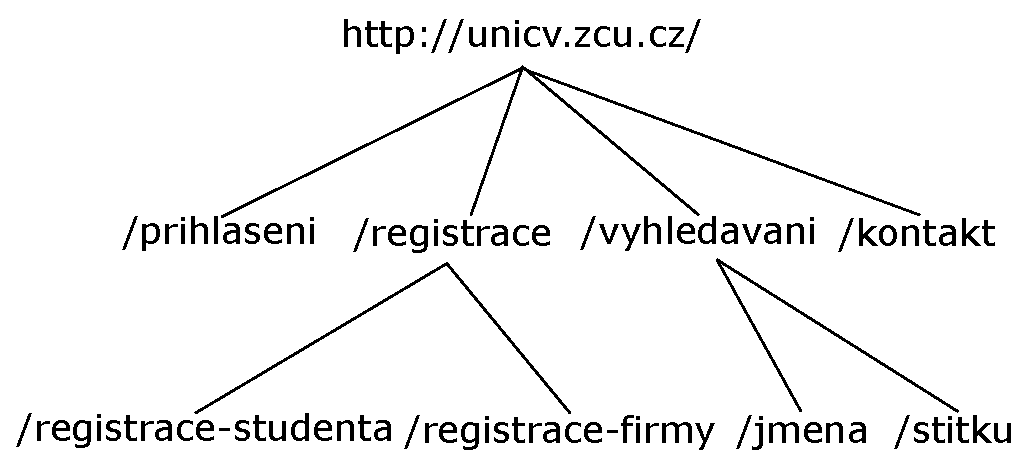
\includegraphics[width=200px]{url_tree.eps}}
\caption{Ukázka stromu webových stránek}
\label{obr.url_stack}
\end{figure}
Získávání stromu je postaveno na strukturách zásobník a datové pole. V zásobníku se ukládají URL pro další provádění a úroveň zanoření (je možné pomocí parametru \textit{-l N}, kde N je hloubka zanoření, definovat, do jaké \uv{hloubky}, se budou odkazy prohledávat). Na referenčním obrázku \ref{obr.url_stack} vidíme, že zanoření úrovně 0 je stránka \textit{http://unicv.zcu.cz}, zanoření úrovně 1 jsou podstránky \textit{/prihlaseni, /registrace, /vyhledavani, /kontakt} a tak dále.

\subsection{Funkce zásobníku}
\begin{figure}[h!]
\centering{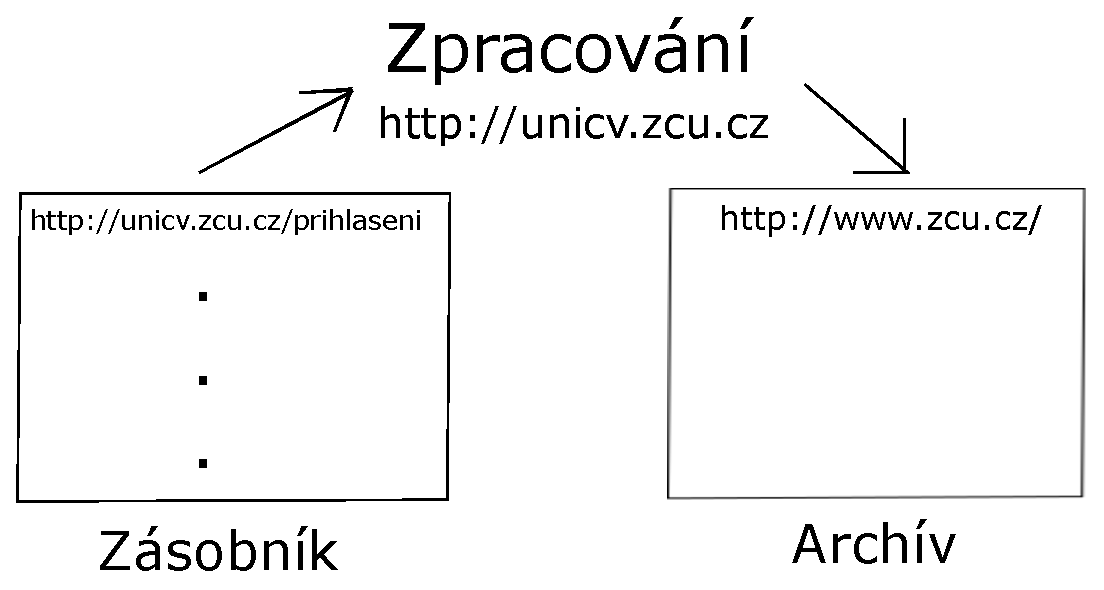
\includegraphics[width=250px]{stack_example.eps}}
\caption{Ukázka stromu webových stránek}
\label{obr.url_tree}
\end{figure}
Do zásobníku jsou ukládány instance třídy \textit{Parser::StackItem} (tato třída je pouze \uv{přepravka}\footnote{Třída, která slouží pouze k uchování dat.}), které mají 2 atributy: URL a hloubku zanoření. Před samotným spuštěním procházení je do zásobníku vložena kořenová stránka (\\v našem případě \textit{http://unicv.zcu.cz}). Následně je spuštěn cyklus, který běží dokud zásobník není prázdný. Pokud stránku zpracujeme (včetně odkazů a formulářů), je uložena do pole historie. Každá nově přidávaná stránka do zásobníku je ověřována proti zásobníku i proti historii, aby nebyla jedna stránka procházena 2x.

\subsection{Získávání a uchovávání odkazů}
Při vytváření URL stromu webových stránek se ihned prochází načtené stránky a zjišťují se formuláře a odkazy na dané stránce. Pro uchování a následné zpracování se využívají 2 pomocné třídy:
\begin{itemize}
\item \textit{Parser::AContainer} - uchovává odkazy a parametry
\item \textit{Parser::FormContainer} - uchovává formuláře, metodu odesílání a jejich parametry
\end{itemize}
Při nalezení nového formuláře nebo odkazu jsou nejprve data porovnávána s poli ve třídě. Pokud již pole obsahuje formulář nebo odkaz, jsou tyto rozšiřovány, což je vidět u příkladu \ref{equals_classes2}, který ukazuje jednoduchost porovnání (za zmínku stojí i aliasování metod, které je řešeno takto: \textit{alias eql? ==}).

\begin{lstlisting}[label=equals_classes2,language=Ruby, caption=Porovnání dvou instancí třídy FormContainer]
# Equals method for comparing
# @param [FormContainer] another_form_container Another form container
# @return [boolean] True or false
def ==(another_form_container)
   # Action URL
   return @action != another_form_container.action && @type != another_form_container.type &&  @params != another_form_container.params
end

# Alias for ==
alias eql? ==
\end{lstlisting}

\subsection{Normalizace URL}
Na webové stránce máme relativně hodně možností jak zapisovat různé odkazy, od relativních cest \textit{./}, přes absolutní \textit{http://server.cz/index.php?action=nova}, až k pouhým \uv{skokům} na stránce \textit{$\#$novinky}. Veškeré tyto URL je potřeba normalizovat, ověřit server (pokud odkazy směřují mimo naší doménu, nejsou použity dále), získat data a odstranit nepotřebné části URL adresy. Při spuštění skriptu můžeme definovat \uv{wildcardování} domén, což znamená, že zadáme doménu prvního řádu: \textit{http://zcu.cz} a pokud je povoleno, bude skritp indexovat i domény vyšších řádů, například \textit{http://unicv.zcu.cz}. V následující tabulce je ukázka případů, kde kořenová doména je \textit{http://unicv.zcu.cz/}:

\begin{table}[!h]
\centering
\begin{tabular}{|l|l|}
\hline
\bf URL v odkazu & \bf Normalizovaná URL \\
\hline
\hline
./index.php?action=help &  http://unicv.zcu.cz/index.php?action=help \\
\hline
$\#$novinky & http://unicv.zcu.cz/$\#$novinky \\
\hline
unicv.zcu.cz/index.php?action=user & http://unicv.zcu.cz/index.php?action=user \\
\hline
http://www.seznam.cz/ & \bf Chybná URL - mimo zadaný server \\
\hline
\end{tabular}
\label{tab:url}
\caption{Příklady normalizování URL}
\end{table}

Prvním krokem bylo nalezení již hotového řešení a výsledek byl překvapující. Ruby po provedení výchozí instalace obsahuje knihovnu \textit{uri}, která umožňuje požadované věci a umí s URL i velice snadno pracovat:

\begin{lstlisting}[label=equals_classes,language=Ruby, caption=Normalizování URL pomocí třídy URI]
# Spojeni 2 URL
url = URI.join("./index.php?action=help#fragment", "http://unicv.zcu.cz/") 
# http://unicv.zcu.cz/index.php?action=help#fragment

# Odstraneni fragmentu
url.fragment = nil
# http://unicv.zcu.cz/index.php?action=help

# Ziskani parametru
url.query
# {:action => "help"}
\end{lstlisting}

\section{Získání URL vectoru stránky}
Pro porovnání délky / obsahu stránek jsem vytvořil modul \textit{URLVector} (modul není třída), který má tři funkce:
\begin{enumerate}
\item Získání vektoru z HTML stránky
\item Odečtení dvou vektorů
\item Získání váhy vektoru
\end{enumerate}
URL vektor je běžná \textit{Hash}\footnote{Klíč - hodnota, v Ruby se klíči říká \textit{symbol}, který vždy začíná \uv{:}} struktura s pevně danými klíči, které jsou názvy elementů viz ukázka html stránky \ref{urlvector} a vektoru \ref{geturlvector} z ní získaného.
\begin{lstlisting}[label=urlvector,language=HTML, caption=HTML stránka]
<html>
   <head>
      <title>Music blog</title>
   </head>
   <body>
       <h1>My music blog</h1>
       <div class="song">
           <strong>Song name</strong>
             ...
       </div>
        ....
   </body>
</html>
\end{lstlisting}

\begin{lstlisting}[label=geturlvector,language=Ruby, caption=Získaný URL vektor]
url_vector = {
     :html => 1, :head => 1, :title => 1, 
     :body => 1, :h1 => 1, :div => 50, :strong => 50
}
\end{lstlisting}


\section{Testování se zapnutými chybovými direktivami pro PHP}
Testování se zapnutými chybovými direktivami je postaveno na principu, že se do parametrů postupně přidá uvozovka, která \uv{zničí} SQL dotaz, v tomto dotazu bude tudíž uvozovka navíc a tento dotaz se nepodaří provést a PHP preprocesor zahlásí chybu. Na stránce jsou tyto chyby následně vyhledávány:
\begin{itemize}
\item do verze PHP 5.2 - mysql$\_$error
\item od verze PHP 5.2 - php notice pro nesprávné použití \textit{while} (v konstrukcích iterací výsledky) nebo pro přístup k asociovaným polím, které neexistují.
\end{itemize}
Pokud je nějaká tato chyba na stránce nalezena, existuje zde vysoká pravděpodobnost, že se podařil SQL injection a tudíž byl SQL dotaz modifikován.

\section{Testování a výměna parametrů}
Testování bez zapnutých direktiv není jednoznačné a výsledky je třeba ověřit ještě ručně. Pro porovnání výsledků s nahrazením parametrů se používají 3 možné případy:
\begin{enumerate}
\item \textit{'} - \uv{rozbití} SQL dotazu
\item \textit{' --} - zakomentování zbytku SQL příkazu
\item \textit{' OR '1' = '1} - logická pravda
\end{enumerate}
U všech je nutné počítat i s jejich \uv{"} - dvojitou uvozovkovou variantou, takže výsledek je  máme 6 získaných stránek.

\subsection{Testování výsledků formulářů}
Formuláře se obecně používají na běžných webových stránkách ke 3 účelům:
\begin{enumerate}
\item Přihlašování
\item Vyhledávání 
\item Filtrování
\end{enumerate}
Pokud se \uv{podvodný} vstup dostane do dotazu, bude mít u každého typu formuláře jiný výsledek, proto se musí otestovat stránka jinak. Máme tudíž 4 webové stránky a vektor prvků na stránce. Vezmeme-li si možné situace, uvidíme, co se s vektory bude dít oproti bezchybnému průběhu.

\begin{itemize}
\item \textbf{Přihlašování}
\begin{enumerate}
\item Snížení počtu prvků na stránce, často přesměrování na nový formulář s hláškou, že chybný požadavek nelze zpracovat, protože SQL dotaz nebylo možno provést.
\item Velká změna při nahrazení v položce \uv{jména}. Díky zakomentování dotazu bude uživatel autorizován a bude přesměrován na stránku s jiným obsahem, zbytek SQL dotazu bylo zakomentováno popřípadě nastala logická pravda, tudíž vždy vrací výsledek.
\item To samé jako v bodě 2)
\end{enumerate}
\item \textbf{Vyhledávání}
\begin{enumerate}
\item Snížením počtu prvků na 0 dotaz nevrátí žádný výsledek = snížení počtu elementů stránky.
\item Zvýšení počtu elementů, může být dosti zásadní (vypisují se všechny prvky) nebo menší (přibudou položky ve stránkování).
\end{enumerate}
\end{itemize}
Z výše zmíněného vyplývá, že je třeba určit všechny možnosti a zjistit značné rozdíly dle modelu chování, protože nejsme schopni strojově rozpoznat, jaký formulář testujeme.

\subsection{Testování výsledků odkazů}
Odkazy se testují na stejném principu jako formuláře, tj. hledají se změny obsahu pomocí vektoru elementů na stránce.

\subsection{Insert-into metoda}
Tato metoda vyžaduje předchozí zásah administrátora nebo vývojáře, je totiž nucen předem vytvořit tabulku \textit{sid\_log} (jejíž definice je ve složce \textit{sql\_dump}). Po spuštění testu je do každého dotazu přidávána struktura \textit{'; INSERT INTO sid\_log(param) VALUE(param\_name)}. Tudíž pokud dotaz projde, je do tabulky přidáno jméno parametru, který tento vstup umožnil. Odpovědné osobě následně stačí tuto tabulku projít po dokončení testu.

\subsection{Drop-All metoda}
Do každého dotazu je přidána direktiva \textit{'; DROP ALL tables; ' --} nebo \textit{'; TRUNCATE ALL tables; ' --}, která způsobí vymazání všech tabulek. Pokud tento dotaz projde, změna obsahu bude skutečně zásadní, popřípadě bude zobrazena stránka 500 (služba je nedostupná). Tato metoda je \textit{opravdu destruktivní}, protože smaže opravdu vše...


\chapter{Porovnání s existujícími nástroji}
\section{Jak probíhalo testování?}
Testování probíhalo na vzorové stránce, která byla připojena na databázi s katalogem hudby (jako v ukázkovém případě). Testovací stránka obsahovala 4 formuláře (2x POST, 2x GET) a odkazy. Polovina parametrů byla nezabezpečených, tudíž mohli být napadnuty. V testu není uveden nástroj od firmy Acunetix - \textit{Web Vulnerability Scanner}, který je pouze pro OS Windows a je placený!

\section{OWASP ZAP}
\subsection{Co je OWASP ZAP?}
\textit{The Open Web Application Security Project} je celosvětová nezisková charitativní organizace, jejíž cílem je zvýšit zabezpeční softwarových řešení, veškeré jejich snahy jsou cíleny na zviditelnění možností bezpečnostních opatření, veškeré materiály, knihy a software, který je vyvíjen je zdarma. 

\begin{figure}[h!]
\centerline{\includegraphics[width=325px]{./examples/owasp.jpeg}}
\caption{https://www.owasp.org/}
\label{owasp}
\end{figure}

\subsection{OWASP ZAP}
\textit{OWASP Zed Attack Proxy Project} je penetrační test pro nalezení bezpečnostních chyb ve webových aplikacích, umožňuje jak manuální kontrolu tak automatické testy. Je k dispozici zdarma: \textit{https://code.google.com/p/zaproxy/}.

\subsection{Nalezené výsledky}
OWASP na testovací stránce nezjistil vůbec žádné problémy typu SQL injection, i když byly zapnuty chybové direktivy. Detekoval ovšem dalších plno problémů s procházením adresářů či špatném zasílání hlaviček.

\section{SQLMap}
\textit{SQLMap - Automatic SQL Injection and database takeover tool}, tato chytrá utilita byla zajímavější než výše předchozí OWASP. Je napsána v jazyce Python a je zdarma k dispozici na \textit{http://sqlmap.org/}. 

\subsection{Nalezené výsledky}
Nepodařilo se mi SQL Map přesvědčit, aby stránky prohledával sám (jako to dělá OWASP), ale při nalezení nezabezpečeného vstupu se ukázal jako výborný pomocník (jak už název napovídá) k převzetí databáze, což se na nezabezpečeném vstupu povedlo bez problémů.

\section{OWASP / SID + SQLMap}
SQLMap a OWASP / SID dohromady tvoří zajímavý nástroj pro detekci a následné \uv{zneužití} SQL injection chyby. OWASP by byl využit pro zjištění všech možných vstupů, které by následně SQL Map otestoval, které je značné množství a SQL Map provádí testy opravdu dlouho. Při využití SIDu a SQL Mapu bude tento čas menší. Při testech SID + SQL Map na vlastním serveru jsem získal všechny tabulky a data z nich.

\chapter{Ukázky}
\subsection{Stažení a instalace}
SID je možné se zdrojovými kódy stáhnout z GIT repozitáře, který je umístěn na serveru GitHub, kde byl v rámci bakalářské práce vyvíjen. Repozitář je read-only, takže je možné ho standartní cestou naklonovat. Dále je přiložen soubor \textit{Gemfile} a \textit{Rakefile}. První ze souborů umožňuje automatické stažení potřebných balíčků (tzv. \textit{Gemů}) pro spuštění programu. Druhý (\textit{Rakefile}) je pro automatické spuštění testů, ze složky \textit{test}. Celý postup je uveden v následující části \ref{SID_instalace}.
\begin{lstlisting}[label=SID_instalace,language=Bash, caption=Instalace]
# Klonovani repozitare
git clone git@github.com:Strnadj/SID.git SID

# Presun do slozky penetracniho testu
cd SID/PenTest

# Stazeni potrebnych balicku
bundle

# Spusteni vsech testu - volitelna moznost
rake

# Presun do slozky se spustitelnou binarkou
cd bin/

# Spusteni testu
./pentest 

\end{lstlisting}
Pokud vše proběhlo správně, zobrazí se nápověda v příkazové řádce s možnými parametry. Jediný povinný parametr je \textit{-u}, kterým zadáváme URL, která se bude zpracovávat. Ostatní parametry jsou nepovinné.

\subsection{Ukázka spuštění}
Pro základní spuštění použijeme následující příkaz:
\begin{lstlisting}[label=SID_run,language=Ruby, caption=Spuštění testu]
./pentest -u http://localhost/test/ -d true -e false
\end{lstlisting}
Používáme tři parametry:
\begin{enumerate}
\item \textit{-u} - URL testované stránky
\item \textit{-d} - tzv. \textit{debug/verbose} mód, který vypisuje veškeré informace o probíhajícím testu
\item \textit{-e} - nastavení zobrazování chyb na serveru, pokud uvedeme false tak jsou direktivy vypnuté a porovnává se obsah
\end{enumerate}
Pokud test spustíme bez parametrů zobrazí se nápověda se seznamem parametrů, které můžeme použít a jejich popisem.

\subsection{Identifikace podezdřelé proměnné}
Pokud test nalezne proměnnou, která je podezdřelá na SQL injection, je přehledně vypsána i s testovacími URL, které byly použity. Administrátor následně může tyto URL zkontrolovat a zkontrolovat parametry (pro identifikaci ve zdrojových kódech můžeme využít například grep).
\begin{figure}[h!]
\centerline{\includegraphics[width=250px]{./examples/SID-success.png}}
\caption{Úspěšné nalezení nezabezpečeného parametru}
\label{chart.attack}
\end{figure}

\chapter{Závěr}
I přes pokus o zobecnění chování změny parametrů, které jsou náchylné právě k SQL injection není možné ve všech ohledech jistě říci, že tyto parametry jsou nechráněné při ověřování porovnání obsahu stránky. Webových aplikací a stránek je nepřeberné množství a každá se chováním trochu odlišuje. I přes testování na vlastních testovacích stránkách a na vzorové stránce společnosti Acunetix (\textit{http://testphp.vulnweb.com/}) se mi podařilo detekovat značné množství výskytů této chyby. I přesto stačí tato chyba pouze jedna a je problém, proto bych při skutečném testování použil kombinaci všech možných dostupných nástrojů (určitě bych i zvažoval zakoupení komerčních nástrojů), tak manuální procházení zdrojových kódů (minimálně částí, týkajících se zpracování těchto požadavků). Rozhodně bych rád tento penetrační test vyvíjel dále, jedním z dalších rozšíření by bylo procházení JavaScriptových souborů pro hledání Ajaxových požadavků a jejich testování a testování při aktivním přihlášení. Ze subjektivního hlediska práce byla velice zajímavá, jak z hlediska jazyka ruby tak i parsování stránek. Penetrační test je pouze pro testovací účel, doufám, že nebude nikdy využit k nelegálním účelům.

\begin{thebibliography}{9}
\addcontentsline{toc}{chapter}{Použitá literatura a zdroje}
\bibitem{owasp}{\em OWASP comunity}
	{\bf OWASP Wiki} \\
	\texttt{https://www.owasp.org/}

\bibitem{soom.cz}{\em Komunitní server}
	{\bf Soom.cz}\\
	\texttt{http://www.soom.cz/}

\bibitem{ruby}{\em Ruby comunnity}
	{\bf Ruby doc}\\
	\texttt{http://www.ruby-lang.org/en/documentation/}

\bibitem{LearnRubyHardWay}{\em E-Book} {\bf Learn Ruby The Hard Way}\\
	\texttt{http://programming-motherfucker.com/}

\bibitem{HackingBezTajemstvi}{\em Joel Scambray, Stuart McClure, George Kurtz}
               {\bf Hacking bez tajemství} \\
           	Computer Press, 2010

\bibitem{php}{\em The PHP Group}
	{\bf PHP - Documentation}\\
	\texttt{http://php.net/manual/en/}

\bibitem{exploitdb}{\em Offensive Security}
	{\bf Exploit-Db}\\
	\texttt{http://www.exploit-db.com/webapps/}

\bibitem{backtrack}{\em Linux Penetration Distribution} {\bf BackTrack 5}\\
	\texttt{http://www.backtrack-linux.org/}


\end{thebibliography}
\end{document}